%-------------------------
% Resume in Latex
% Author : Vladimir SIRGHI
%------------------------

% supports 10, 11, 12pt font sizes
% letterpaper = 8.5in x 11in
\documentclass[letterpaper,11pt]{article}

% set margins
\usepackage[
    left=0.5in,
    right=0.5in,
    top=0.4in,
    bottom=0.4in,
]{geometry}
\usepackage{latexsym}
\usepackage{titlesec}
\usepackage{marvosym}
\usepackage[usenames,dvipsnames]{color}
\usepackage{verbatim}
\usepackage{enumitem}
\usepackage[hidelinks]{hyperref}
\usepackage{fancyhdr}
\usepackage[english]{babel}
\usepackage{tabularx}
\usepackage{hyphenat}
\usepackage{fontawesome}
\usepackage{enumitem}
\input{glyphtounicode}
\usepackage{parskip}
\usepackage{graphicx}
\usepackage{etoolbox}  % for conditional logic
\usepackage{csquotes}
\usepackage{footmisc}

\renewcommand{\footnotesize}{\scriptsize} % réduit la taille des footnotes

% is_long_version = true will render more detailed resume
\newtoggle{is_long_version} % Define the boolean variable
\ifdefined\shortversion
  \settoggle{is_long_version}{false}
\else
  \settoggle{is_long_version}{true}
\fi

\pagestyle{fancy}

% clear all header and footer fields
\fancyhf{}
\fancyfoot{}
% remove lines between header/footer
\renewcommand{\headrulewidth}{0pt}
\renewcommand{\footrulewidth}{0pt}

\urlstyle{same}

% don't stretch text to fill the entire line
\raggedbottom
\raggedright
% remove horizontal padding from table cells
\setlength{\tabcolsep}{0in}

% Section heading formatting
\titleformat{\section}{
  \scshape\raggedright\large
}{}{0em}{}[\color{black}\titlerule]

% Ensure that generate pdf is machine readable/ATS parsable
\pdfgentounicode=1

%%% Set spacing %%%
% set vertical spacing between sections
\titlespacing*{\section}
{0pt} % left indent
{2pt} % spacing above
{2pt} % spacing below

\linespread{1.01}  % line spacing
\setlength{\parskip}{0pt} % paragraph spacing

% bullet list spacing
\setlist[itemize]{itemsep=0pt} % vertical spacing between bullets
\def\vspaceAfterBullets{1pt} % vertical spacing after bullet lists
\def\bulletIndent{15pt} % indent of bullet lists

% set bullet list symbol formatting
\setlist[itemize,1]{label=$\vcenter{\hbox{\tiny$\bullet$}}$}
\setlist[itemize,2]{label=$\vcenter{\hbox{\tiny$\bullet$}}$}
\setlist[itemize,3]{label=$\vcenter{\hbox{\tiny$\circ$}}$}

%-------------------------
% Custom commands

\newcommand{\bulletItem}[1]{
  \item\small{
    {#1}
  }
}

% company name -- location
\newcommand{\companyNameAndLocationHeading}[2]{
  \item
    \begin{tabular*}{1.0\textwidth}[b]{l@{\extracolsep{\fill}}r}
      \textbf{#1} & #2
    \end{tabular*}
}

% job title -- date
\newcommand{\titleAndDateHeading}[2]{
    \item
    \begin{tabular*}{1.0\textwidth}[b]{l@{\extracolsep{\fill}}r}
      {\bfseries\itshape\small #1} & \itshape\small #2
    \end{tabular*}
}

% project name -- date
\newcommand{\resumeProjectHeading}[2]{
    \item
    \begin{tabular*}{1.0\textwidth}[b]{l@{\extracolsep{\fill}}r}
      \small#1 & #2
    \end{tabular*}
}

\newcommand{\sectionListStart}{\begin{itemize}[leftmargin=0pt, label={}]}
\newcommand{\sectionListEnd}{\end{itemize}}

\newcommand{\outerBulletListStart}{\begin{itemize}[leftmargin=\bulletIndent]}
\newcommand{\outerBulletListEnd}{\end{itemize}\vspace{\vspaceAfterBullets}}


\newcommand{\innerBulletListStart}{\begin{itemize}[leftmargin=\bulletIndent]}
\newcommand{\innerBulletListEnd}{\end{itemize}}

% blue colored hyperlinks
\newcommand{\bref}[2]{\href{#1}{\color{blue}{#2}}}


%-------------------------------------------
%%%%%%  RESUME STARTS HERE  %%%%%%%%%%%
%
\begin{document}

%---------- HEADING ----------
% Header
\def\spaceAfterLogo{0.5pt}
 \begin{center}
   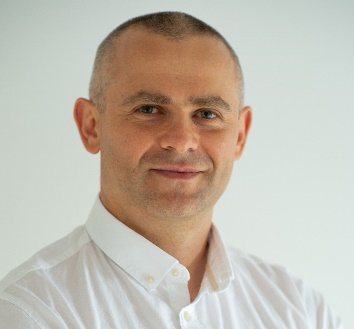
\includegraphics[width=3cm]{../ressources/photo/cv_photo.jpg} \\[1em]
   \textbf{\LARGE Vladimir Sirghi} \\ \vspace{3pt}
   \small
   \faLinkedinSquare \hspace{\spaceAfterLogo} \href{https://www.linkedin.com/in/vladimir-sirghi/}{linkedin}
   $|$
   \faEnvelope \hspace{\spaceAfterLogo} \href{mailto:sirghivladimir@gmail.com}{sirghivladimir@gmail.com}
   $|$
  %  \faMobile \hspace{\spaceAfterLogo} \href{tel:+33638608085}{(+33) 638.60.80.85}
  %  $|$
   \faGithub \hspace{\spaceAfterLogo} \href{https://github.com/slalomeset}{github.com/slalomeset}
   $|$
   \faMapMarker \hspace{\spaceAfterLogo} \href{https://www.google.com/maps/place/Annecy}{Annecy, France}
 \end{center}

%----------- SUMMARY -----------
\iftoggle{is_long_version}
{
  \section{Summary}
  \small Senior Embedded Software Engineer with 8+ years of experience in semiconductor and automotive systems. Specializes in bare-metal C, firmware bring-up, hardware qualification, and safety-critical verification across ARM Cortex-M and FPGA platforms.}{}
\vspace{1em} % Add space here
%----------- EXPERIENCE -----------

\section{Experience}
\sectionListStart

\companyNameAndLocationHeading {\bref{https://www.st.com/}{STMicroelectronics}}{Le Bourget-du-lac, France}
\titleAndDateHeading
{Senior Embedded Software Engineer}{March 2022 \textbf{--} Present}
\outerBulletListStart
\bulletItem{Develop safety-critical firmware for automotive Ultra-Wideband (UWB) systems on ARM Cortex-M and FPGA platforms.}
\bulletItem{Improve software reliability with CMocka unit tests and Python/Gauge automated integration tests.}
\bulletItem{Support project predictability through active participation in Agile cycles and detailed technical documentation.}
\bulletItem{Coordinate with multidisciplinary engineering teams to maintain system alignment and quality standards.}
\bulletItem{Develop Python-based automated tests and monitor execution through Jenkins CI/CD pipelines.}
\bulletItem{\textbf{Key Contributions:}}
\begin{itemize}
  \item Develop and maintain embedded firmware for UWB SoC HTOL (High-Temperature Operating Life) qualification, delivering successive releases with qualification test scenarios.
  \item Port HTOL firmware across board and silicon revisions and support qualification runs with Quality, RF, and external partners.
  \item Coordinate verification efforts to support timely "Go" decisions for silicon pattern generation.
  \item Develop the low-level interface of a ROS/PlotJuggler diagnostic module adopted as a standard tool for system analysis.
  \item Design power profiling firmware to support measurement and optimization of SoC energy efficiency.
\end{itemize}
\outerBulletListEnd
\vspace{1em} % Add space here

\companyNameAndLocationHeading {\bref{https://www.st.com/}{STMicroelectronics}}{Le Bourget-du-lac, France}
\titleAndDateHeading
{Verification Lead and Development (Pre-PG)}{March 2024 \textbf{--} December 2024}
\outerBulletListStart
    \bulletItem{\textbf{Methodology:} Lead Agile sprint planning and milestone tracking, coordinating team efforts around project targets and requirements.}
    \bulletItem{\textbf{Engineering:} Contribute to feature development, debugging, and code reviews to deliver reliable technical outputs.}
\outerBulletListEnd

\companyNameAndLocationHeading
{\bref{https://atos.net/}{Atos}}{Grenoble, Auvergne-Rhône-Alpes, France}
\titleAndDateHeading
{Safety Test Engineer | CMOS Image Sensors}{October 2020 \textbf{--} February 2022}
\outerBulletListStart
\bulletItem{Support compliance with automotive safety standard ISO 26262 by developing Python-based validation suites for CMOS image sensors.}
\bulletItem{Validate hardware/software safety mechanisms (ASIL) to verify system integrity, including:}
\innerBulletListStart
    \bulletItem{\textbf{Core monitoring:} MCU watchdog, stack integrity, lockstep, and clock Built-In Self-Test (BIST).}
    \bulletItem{\textbf{Memory \& Data:} Memory parity/ECC, CRC program protection, and OTP integrity.}
    \bulletItem{\textbf{Environment:} Voltage, thermal monitoring, and periodic crack detection blocks.}
\innerBulletListEnd
\bulletItem{Collaborate within an Agile framework to document formal test specifications and produce detailed safety reports for certification purposes.}
\bulletItem{Maintain quality through Git version control and Jenkins CI/CD automation.}
\outerBulletListEnd
\vspace{1em}

\newpage
\companyNameAndLocationHeading
{\bref{https://www.st.com/}{STMicroelectronics}}{Grenoble, Auvergne-Rhône-Alpes, France}
\titleAndDateHeading
{Test Engineer}{September 2018 \textbf{--} August 2020}
\outerBulletListStart
\bulletItem{Developed Python scripts for unitary, integration, and system tests on hardware and firmware components.}
\bulletItem{Documented test requirements and reported test results.}
\bulletItem{Used Git for code versioning.}
\bulletItem{Resolved tickets and issues affecting hardware and firmware components.}
\outerBulletListEnd
\vspace{0.25em}

\companyNameAndLocationHeading
{\bref{https://www.defense.gouv.fr/terre}{French Army}}{France}
\titleAndDateHeading
{Team Lead and Electro-mechanical Specialist}{September 2010 \textbf{--} August 2018}
\outerBulletListStart
\bulletItem{Maintained the operational readiness of critical energy infrastructure in high-pressure environments.}
\bulletItem{Mentored and trained junior technicians, promoting team cohesion and technical excellence.}
\bulletItem{Applied preventive and corrective maintenance protocols to support continuous power for strategic networks.}
\bulletItem{Built a culture of responsibility and precision to support mission-critical operations.}
\outerBulletListEnd
\sectionListEnd
\vspace{0.25em} % Add space here

%----------- EDUCATION -----------
\section{Education}
\sectionListStart
\companyNameAndLocationHeading
{\bref{https://scem-eset.univ-smb.fr/}{Savoie Mont Blanc University}}{Le Bourget-du-Lac, France}
\titleAndDateHeading
{\bref{https://github.com/slalomeset/diplomas/blob/main/master.pdf}{Master's Degree in \enquote{Electronics of Embedded Systems and Telecommunications}}}{September 2018 \textbf{--} August 2020}

\companyNameAndLocationHeading
{\bref{https://sup-fc.univ-fcomte.fr/informatique}{University of Franche-Comté}}{Bourgogne-Franche-Comté, France}
\titleAndDateHeading
{Bachelor in \enquote{Computer Science}}{September 2020 \textbf{--} August 2021}

\companyNameAndLocationHeading
{\bref{https://www.univ-tlse3.fr/decouvrir-nos-diplomes/licence-parcours-eea-fondamental-eea-f}{Toulouse 3 University \enquote{Paul Sabatier}}}{Toulouse, France}
\titleAndDateHeading
{\bref{https://github.com/slalomeset/diplomas/blob/main/bachelor.pdf}{Bachelor in \enquote{Electronics, Electrical Engineering and Automation.}}}{September 2016 \textbf{--} August 2018}

\companyNameAndLocationHeading
{\bref{https://www.cned.fr/}{CNED \enquote{Centre National d'Enseignement à Distance}}}{Avignon, France}
\titleAndDateHeading
{\bref{https://github.com/slalomeset/diplomas/blob/main/bts.pdf}{BTEC HND in \enquote{Electrical Engineering and Electronics }}}{September 2014 \textbf{--} August 2016}

\companyNameAndLocationHeading
{\bref{https://www.armyacademy.ro/engleza/fmm.php}{\enquote{Nicolae Balcescu} Land Forces Academy }}{Sibiu, Romania }
\titleAndDateHeading
{\bref{https://github.com/slalomeset/diplomas/blob/main/military_academy.pdf}{ Bachelor's Degree in Management of Military Organizations }}{September 2002 \textbf{--} August 2006}
\sectionListEnd

\vspace{0.25em} % Add space here

\section{Languages}
\sectionListStart
\bulletItem{\textbf{English:}{ Professional} \bref{https://github.com/slalomeset/certificates/blob/main/toeic_english.pdf}{[TOEIC certificate]} }
\bulletItem{\textbf{French:}{ Native}}
\bulletItem{\textbf{Romanian:}{ Native}}
\sectionListEnd
\vspace{0.25em} % Add space here

%----------- Professional Training -----------
\section{Professional Trainings}
\outerBulletListStart
\bulletItem{Writing secure firmware}
\bulletItem{ISO26262 in Product Development}
\bulletItem{Automotive Safety HW ISO26262}
\bulletItem{Object Oriented Programming in C++}
\bulletItem{General Imaging Concepts \& Integration}
\bulletItem{Understanding Image Sensor Characterization}
\bulletItem{Indirect Time Of Flight}
\bulletItem{Image Sensors Architecture}
\bulletItem{Algorithms for Image Analysis}
\bulletItem{Imaging Signal Processing Algorithms}
\outerBulletListEnd
\vspace{0.25em} % Add space here

%----------- SKILLS -----------
\section{Technical Expertise}
\sectionListStart
\bulletItem{\textbf{Core:} Embedded C (Advanced), Bare-metal, ARM Cortex-M, ISO 26262 (Automotive Safety).}
\bulletItem{\textbf{Scripting \& Quality:} Python, Bash, Jenkins CI/CD (User), CMocka, Gauge, Unit/Integration Testing.}
\bulletItem{\textbf{Tools \& Protocols:} Git, CMake, OpenOCD, ROS, GDB, I2C, SPI, UART, CAN, SWD.}
\bulletItem{\textbf{AI-Assisted Engineering:} GitHub Copilot, Prompt Engineering for Embedded Constraints, AI Code Auditing.}
\sectionListEnd
\vspace{1em} % Add space here

%-------------------------------------------
\end{document}
